\documentclass[border=10pt]{standalone}
\usepackage{tikz}
\usetikzlibrary{patterns}
\usepackage{amsmath}

% ensures a white background in the converted image
\pagecolor{white}

\begin{document}
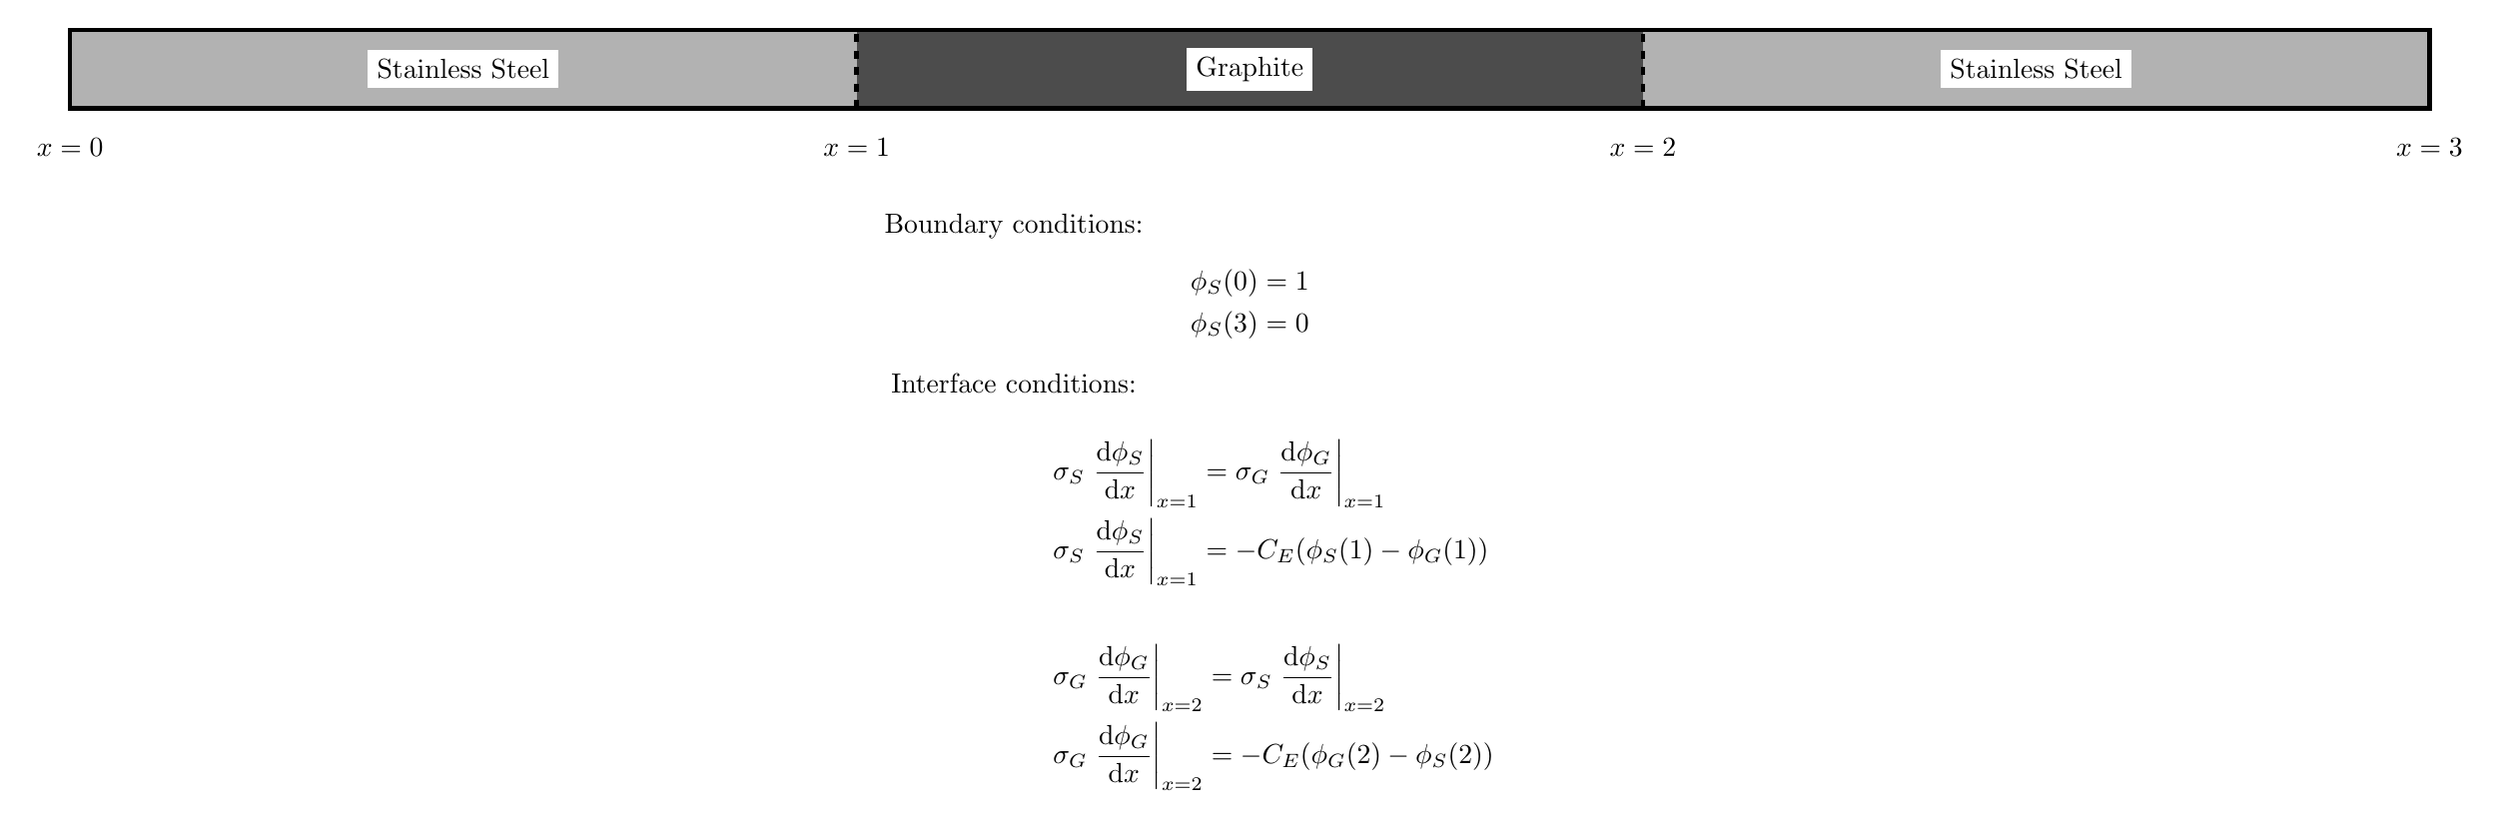
\begin{tikzpicture}
  % draw fills so lines sit on top of them
  \fill [fill=black!30!white] (0, 0) rectangle (10, 1);
  \fill [fill=black!70!white] (10, 0) rectangle (20, 1);
  \fill [fill=black!30!white] (20, 0) rectangle (30, 1);
  % outlines
  \draw [ultra thick] (0, 0) rectangle (30, 1);
  \draw [ultra thick, dashed] (10, 0) -- (10, 1);
  \draw [ultra thick, dashed] (20, 0) -- (20, 1);
  % material labels
  \node [fill=white] at (5, 0.5) {Stainless Steel};
  \node [fill=white] at (15, 0.5) {Graphite};
  \node [fill=white] at (25, 0.5) {Stainless Steel};
  % position markers
  \node at (0, -0.5) {$x = 0$};
  \node at (10, -0.5) {$x = 1$};
  \node at (20, -0.5) {$x = 2$};
  \node at (30, -0.5) {$x = 3$};
  % boundary conditions
  \node at (12, -1.5) {Boundary conditions:};
  \node [text width=5cm] at (15, -2.25) {
      \begin{align*}
        \phi_S (0) &= 1 \\
        \phi_S (3) &= 0
      \end{align*}
  };
  % interface conditions
  \node at (12, -3.5) {Interface conditions:};
  \node [text width=5cm] at (15, -6.25) {
      \begin{align*}
        \sigma_S \left. \frac{\text{d} \phi_S}{\text{d} x} \right|_{x = 1} &= \sigma_G \left. \frac{\text{d} \phi_G}{\text{d} x} \right|_{x = 1} \\
        \sigma_S \left. \frac{\text{d} \phi_S}{\text{d} x} \right|_{x = 1} &= -C_E (\phi_S(1) - \phi_G(1))
      \end{align*}
      \begin{align*}
        \sigma_G \left. \frac{\text{d} \phi_G}{\text{d} x} \right|_{x = 2} &= \sigma_S \left. \frac{\text{d} \phi_S}{\text{d} x} \right|_{x = 2} \\
        \sigma_G \left. \frac{\text{d} \phi_G}{\text{d} x} \right|_{x = 2} &= -C_E (\phi_G(2) - \phi_S(2))
      \end{align*}
  };
\end{tikzpicture}
\end{document}
